%!TEX program = pdflatex

\documentclass[11pt,aspectratio=169]{beamer}

% Tema y colores
\usetheme{Madrid}
\usecolortheme{whale}

% Paquetes necesarios
\usepackage[utf8]{inputenc}
\usepackage[spanish]{babel}
\spanishsignitems
\usepackage{tikz}
\usetikzlibrary{shapes,shadows,arrows,positioning,calc}
\usetikzlibrary{babel}
\usepackage{amsmath}
\usepackage{graphicx}
\usepackage{booktabs}
\usepackage{multicol}
\usepackage{hyperref}

\usepackage{fontawesome5}          % Para \faEnvelope etc.
\usepackage{microtype}             % Reduce overfull hbox
\usepackage{newunicodechar}
\newunicodechar{≠}{\ensuremath{\neq}}         % O reemplaza manualmente ≠ por \neq
\tolerance=800           % Más permisivo con justificación
\hbadness=8000           % Ignora boxes "malos" hasta cierto punto
\emergencystretch=3em    % Permite estirar espacios en líneas problemáticas

\hypersetup{
	colorlinks=true,
	linkcolor=blue,
	urlcolor=cyan
}

\tikzset{
    conceptbox/.style={
        rectangle,                % forma básica: rectángulo
        rounded corners=3mm,      % esquinas redondeadas (bastante notorias)
        draw=#1!60,               % borde usa el color base al 60% de saturación/intensidad
        fill=#1!20,               % relleno muy suave (20%) → queda claro y elegante
        thick,                    % borde grueso para que destaque
        minimum height=2cm,       % altura mínima razonable para que no quede apretado
        text width=0.9\linewidth, % ancho útil (deja márgenes laterales bonitos)
        align=left,               % texto alineado a la izquierda (más natural para párrafos)
        inner sep=10pt,           % espacio interior generoso → se lee cómodo
        drop shadow               % sombra suave (efecto de "tarjeta" elevado)
    },
    examplebox/.style={
        rectangle,
        rounded corners=3mm,      % mantiene la misma estética redondeada
        draw=#1!60,
        fill=#1!15,               % relleno aún más claro (15%) para que no compita con conceptbox
        thick,
        minimum height=1.5cm,     % altura más reducida → ideal para ejemplos cortos
        text width=0.9\linewidth,
        align=left,
        inner sep=8pt             % un poco menos espacio interno (queda más compacto)
        % Nota: no lleva drop shadow para diferenciarlo visualmente de conceptbox
    },
    keypoint/.style={
        rectangle,
        rounded corners=2mm,      % esquinas un poco menos redondeadas (más "serias")
        draw=#1!70,               % borde más intenso (70%) para que resalte
        fill=#1!25,               % relleno intermedio (25%) → buen contraste
        thick,
        minimum width=0.4\textwidth, % ancho mínimo → fuerza a que sea más bien ancho
        align=center,             % centrado → muy común en "key points" o conclusiones
        inner sep=6pt             % espacio interno más ajustado (queda conciso)
        % Nota: no lleva altura mínima para adaptarse al contenido
    }
}

% Ejemplos de uso:
%
% \node[conceptbox=blue] {Esto es un concepto importante...};
%
% \node[examplebox=green!70!black] {Ejemplo práctico: ...};
%
% \node[keypoint=orange] {Punto clave: recordar que ...};

% Información del documento
\title[Búsqueda de Información Académica]{Búsqueda y Gestión de Información Académica}
\subtitle{Fundamentos para la investigación universitaria y el trabajo científico}
\author{Edison Achalma}
\institute{
	Corporación Académica Universitaria \\
	CAU - UNSCH
}
\date{\today}

\titlegraphic{
\includegraphics[width=2cm]{images/cau-logo.png}}

\begin{document}
\shorthandoff{"}

% ==================== PORTADA ====================
\begin{frame}
	\titlepage
\end{frame}

% ==================== ÍNDICE ====================
\begin{frame}{Contenido del Curso}
	\tableofcontents
\end{frame}

% ==================== PARTE I: FUNDAMENTOS ====================
\section{Ciencia e Información}

\begin{frame}{¿Qué es la Ciencia?}
	\tikz\node[conceptbox=blue]{
		\textbf{Definición:}\\[0.3cm]
		La ciencia es una \textbf{representación altamente depurada y fiable de la realidad}, generada en el seno de comunidades de expertos mediante \textbf{procedimientos contrastados} y abiertos a la crítica constante.
	};

	\vspace{0.4cm}

	\begin{columns}[T]
		\begin{column}{0.48\textwidth}
			\textbf{Características:}
			\begin{itemize}
				\item Conocimiento \textbf{acumulativo}
				\item Saber \textbf{crítico} y verificable
				\item \textbf{Público} y accesible
				\item \textbf{Fijo} y documentado
			\end{itemize}
		\end{column}
		\begin{column}{0.48\textwidth}
			\textbf{La ciencia se distingue de:}
			\begin{itemize}
				\item Opinión personal
				\item Ideología y propaganda
				\item Pseudociencia
				\item Creencias no verificadas
			\end{itemize}
		\end{column}
	\end{columns}
\end{frame}

% IMAGEN SUGERIDA: Diagrama circular o pirámide mostrando la jerarquía del conocimiento
% (datos → información → conocimiento → sabiduría)
% O imagen conceptual de "a hombros de gigantes"

\begin{frame}{La Ciencia como Construcción Comunitaria}
	\tikz\node[conceptbox=teal]{
		\textbf{``A hombros de gigantes''}
		El nuevo conocimiento se construye sobre la base del conocimiento preexistente. La ciencia avanza mediante la \textbf{construcción colectiva} de comunidades de expertos.
	};

	\vspace{0.1cm}

	\begin{center}
		\begin{tikzpicture}[node distance=1.8cm]
			\node[keypoint=blue] (invest) {\textbf{Investigación}\\Original};
			\node[keypoint=green, right=of invest] (revision) {\textbf{Revisión}\\por Pares};
			\node[keypoint=violet, below=0.3cm of revision] (public) {\textbf{Publicación}\\Acreditada};
			\node[keypoint=orange, left=of public] (uso) {\textbf{Uso y}\\Citación};

			\draw[->,thick] (invest) -- (revision);
			\draw[->,thick] (revision) -- (public);
			\draw[->,thick] (public) -- (uso);
			\draw[->,thick] (uso) -- (invest);
		\end{tikzpicture}
	\end{center}

	\vspace{0.1cm}

	\tikz\node[examplebox=cyan]{
		\textbf{La comunicación es esencial:} Los documentos científicos son el medio que permite que el conocimiento sea público, fijo y fiable.
	};
\end{frame}

% IMAGEN SUGERIDA: Red de nodos interconectados representando la comunidad científica
% O fotografía histórica de científicos colaborando

% =====================================================================
% DIAPOSITIVA 1: Internet Superficial (Surface Web)
% =====================================================================
\begin{frame}{Los Tres Niveles de Internet - 1/3}
	\begin{columns}[T]
		\begin{column}{0.5\textwidth}
			\center
			\tikz\node[conceptbox=blue]{
				\textbf{Internet Superficial}\\
				\textbf{(Surface Web - 30\%)}\\[0.3cm]
				• Páginas indexadas\\
				• Google, redes sociales\\
				• Acceso libre y directo\\
				• Ejemplos: Google, Facebook, YouTube\\
				• \textcolor{red}{Calidad variable}
			};
		\end{column}

		\begin{column}{0.5\textwidth}
			% Aquí va la imagen referencial del Surface Web
			% Sugerencia: captura de buscador Google o redes sociales
			\center
			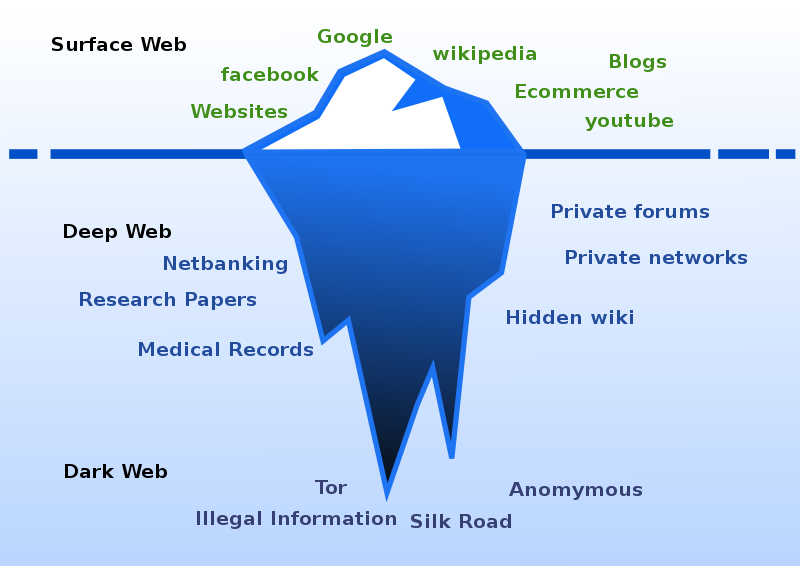
\includegraphics[width=0.9\textwidth,height=0.6\textheight,keepaspectratio]{images/surface_web.png}
		\end{column}
	\end{columns}

\end{frame}

% =====================================================================
% DIAPOSITIVA 2: Internet Profunda (Deep Web)
% =====================================================================
\begin{frame}{Los Tres Niveles de Internet - 2/3}
	\begin{columns}[T]
		\begin{column}{0.5\textwidth}
			\center
			\tikz\node[conceptbox=teal]{
				\textbf{Internet Profunda}\\
				\textbf{(Deep Web - 70\%)}\\[0.3cm]
				• Bases de datos\\
				• Contenido protegido\\
				• Requiere autenticación\\
				• Ejemplos: Bases de datos, Gmail, Dropbox\\
				• \textcolor{green!60!black}{Mayor calidad científica}
			};
		\end{column}

		\begin{column}{0.5\textwidth}
			% Aquí va la imagen referencial del Deep Web
			% Sugerencia: bases de datos académicas, login universidad, bibliotecas digitales
			\center
			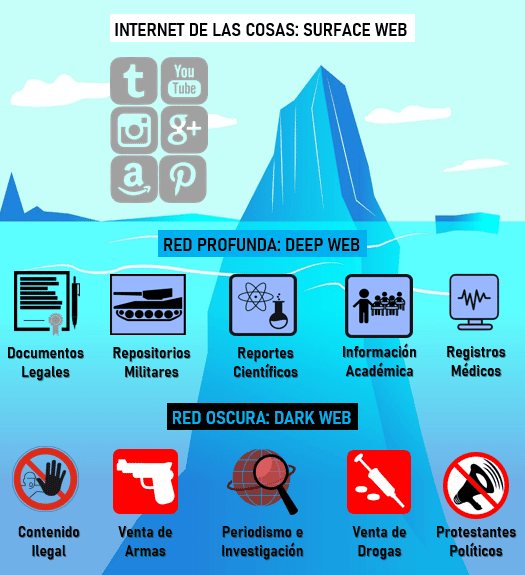
\includegraphics[width=0.9\textwidth,height=0.5\textheight,keepaspectratio]{images/deep_web.png}
		\end{column}
	\end{columns}

	\vspace{0.1cm}
	\tikz\node[examplebox=orange]{
		\textbf{Clave:} La mayoría de la información científica de calidad está en la \textbf{Internet Profunda}, accesible a través de bibliotecas universitarias.
	};
\end{frame}



% =====================================================================
% DIAPOSITIVA 3: Internet Oscura (Dark Web) + mensaje final
% =====================================================================
\begin{frame}{Los Tres Niveles de Internet - 3/3}
	\begin{columns}[T]
		\begin{column}{0.5\textwidth}
			\center
			\tikz\node[conceptbox=gray]{
				\textbf{Internet Oscura}\\
				\textbf{(Dark Web)}\\[0.2cm]
				Redes privadas (Tor)\\
				No recomendado\\
				para fines académicos
			};
		\end{column}

		\begin{column}{0.5\textwidth}
			% Aquí va la imagen referencial del Dark Web
			% Sugerencia: icono de candado, navegador Tor, ambiente oscuro
			\center
			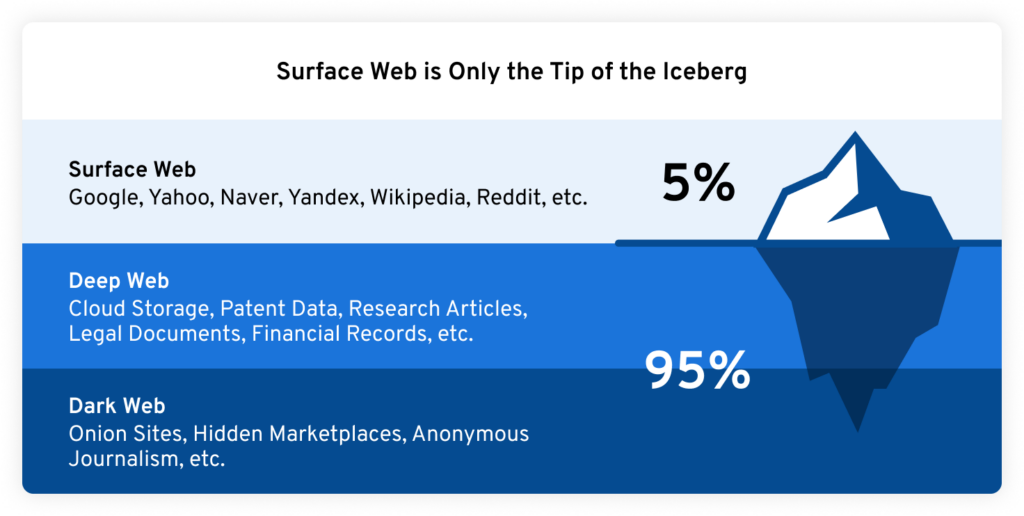
\includegraphics[width=0.9\textwidth,height=0.6\textheight,keepaspectratio]{images/dark_web.png}
		\end{column}
	\end{columns}

\end{frame}

\begin{frame}{Infoxicación: El Desafío Actual}
	\tikz\node[conceptbox=red]{
		\textbf{¿Qué es la infoxicación?}\\[0.3cm]
		Sobrecarga de información que \textbf{dificulta el análisis, selección y uso efectivo} de datos relevantes. El problema no es la falta de información, sino el \textbf{exceso}.
	};

	\vspace{0.1cm}

	\begin{columns}[T]
		\begin{column}{0.48\textwidth}
			\textbf{Características:}
			\begin{itemize}
				\item Cobertura global
				\item Actualización constante
				\item Acceso inmediato
				\item Volumen abrumador
			\end{itemize}
		\end{column}
		\begin{column}{0.48\textwidth}
			\textbf{Consecuencias:}
			\begin{itemize}
				\item Dificultad para discernir
				\item Pérdida de tiempo
				\item Información no confiable
				\item Estrés cognitivo
			\end{itemize}
		\end{column}
	\end{columns}

	\vspace{0.1cm}

	\tikz\node[examplebox=yellow]{
		\textbf{Solución:} Búsqueda \textbf{estratégica} y \textbf{crítica}, no mecánica.
	};
\end{frame}

% IMAGEN SUGERIDA: Persona abrumada frente a múltiples pantallas o flujo de información
% O gráfico mostrando el crecimiento exponencial de datos

% ==================== PARTE II: FUENTES DE INFORMACIÓN ====================
\section{Clasificación y Tipos de Fuentes}

\begin{frame}{Fuentes Primarias vs. Secundarias}
	\begin{columns}[T]
		\begin{column}{0.48\textwidth}
			\tikz\node[conceptbox=green]{
				\textbf{Fuentes primarias}\\[0.3cm]
				\textbf{Información directa y original}\\[0.2cm]
				• Artículos científicos originales\\
				• Tesis y disertaciones\\
				• Informes técnicos\\
				• Datos estadísticos oficiales\\
				• Patentes\\
				• Comunicaciones de congresos
			};
		\end{column}
		\begin{column}{0.48\textwidth}
			\tikz\node[conceptbox=violet]{
				\textbf{Fuentes secundarias}\\[0.3cm]
				\textbf{Información procesada}\\[0.2cm]
				• Manuales y tratados\\
				• Artículos de revisión (reviews)\\
				• Enciclopedias\\
				• Bases de datos bibliográficas\\
				• Índices y catálogos
			};
		\end{column}
	\end{columns}

	\vspace{0.4cm}

	\tikz\node[examplebox=cyan]{
		\textbf{Uso estratégico:} Las secundarias son ideales para \textit{acercamiento inicial}; las primarias para \textit{investigación profunda}.
	};
\end{frame}

% IMAGEN SUGERIDA: Diagrama de flujo mostrando cómo las fuentes primarias
% alimentan las secundarias, y ambas al investigador

\begin{frame}{Tipos de Documentos Científicos}
	\small
	\begin{multicols}{2}
		\textbf{Según su función:}
		\begin{enumerate}
			\item \textbf{Síntesis:} Manuales, tratados, enciclopedias
			\item \textbf{Investigación:} Artículos, monografías, tesis
			\item \textbf{Difusión:} Actas de congresos (proceedings)
			\item \textbf{Técnicos:} Normas, patentes, informes
			\item \textbf{Legales:} Leyes, reglamentos, decretos
		\end{enumerate}

		\columnbreak

		\textbf{Identificadores únicos:}
		\begin{itemize}
			\item \textbf{ISBN:} Libros (13 dígitos)
			\item \textbf{ISSN:} Revistas (8 dígitos)
			\item \textbf{DOI:} Artículos digitales
			\item \textbf{ORCID:} Autores
		\end{itemize}
	\end{multicols}

	\vspace{0.3cm}

	\tikz\node[examplebox=blue]{
		\textbf{Importante:} Conocer el \textbf{tipo de documento} ayuda a elegir la \textbf{herramienta de búsqueda} adecuada.
	};
\end{frame}

% IMAGEN SUGERIDA: Infografía con íconos representando cada tipo de documento
% (libro, revista, documento legal, patente, etc.)

\begin{frame}{Revistas Científicas (Journals)}
	\tikz\node[conceptbox=magenta]{
		\textbf{¿Qué es una revista científica?}\\[0.3cm]
		Publicación periódica donde se publican artículos sometidos a \textbf{revisión por pares (peer-review)}, garantizando calidad y rigor científico.
	};

	\vspace{0.4cm}

	\begin{columns}[T]
		\begin{column}{0.48\textwidth}
			\textbf{Características:}
			\begin{itemize}
				\item Control editorial riguroso
				\item Periodicidad regular
				\item Identificación con ISSN
				\item Indexación en bases de datos
			\end{itemize}
		\end{column}
		\begin{column}{0.48\textwidth}
			\textbf{Tipos de artículos:}
			\begin{itemize}
				\item \textbf{Originales:} Nuevas investigaciones
				\item \textbf{Reviews:} Estado del arte
				\item \textbf{Comunicaciones:} Hallazgos breves
				\item \textbf{Cartas:} Comentarios críticos
			\end{itemize}
		\end{column}
	\end{columns}
\end{frame}

% IMAGEN SUGERIDA: Portada de una revista científica reconocida
% O diagrama del proceso de peer-review

\begin{frame}{Tesis y Trabajos Académicos}
	\tikz\node[conceptbox=teal]{
		\textbf{Documentos académicos que conducen a un título}\\[0.3cm]
		Realizados bajo dirección de expertos, representan la culminación de un proceso formativo y demuestran competencia para generar conocimiento.
	};

	\vspace{0.3cm}

	\begin{columns}[T]
		\begin{column}{0.2\textwidth}
			\tikz\node[keypoint=blue]{
				\textbf{TFG}\\
				Trabajo Fin de Grado\\[0.1cm]
				\small Aplicación de\\
				conocimientos
			};
		\end{column}
		\begin{column}{0.2\textwidth}
			\tikz\node[keypoint=green]{
				\textbf{TFM}\\
				Trabajo Fin de Máster\\[0.1cm]
				\small Iniciación a la\\
				investigación
			};
		\end{column}
		\begin{column}{0.2\textwidth}
			\tikz\node[keypoint=violet]{
				\textbf{Tesis Doctoral}\\
				~\\[0.1cm]
				\small Aportación original al\\
				conocimiento
			};
		\end{column}
	\end{columns}

	\vspace{0.1cm}

	\tikz\node[examplebox=orange]{
		\textbf{Recuperación:} Repositorios institucionales, RENATI, Alicia, Teseo, OATD
	};
\end{frame}

% IMAGEN SUGERIDA: Pirámide mostrando TFG → TFM → Tesis Doctoral
% O fotografía de una ceremonia de graduación doctoral

% ==================== PARTE III: CRITERIOS DE CALIDAD ====================
\section{Evaluación Crítica de Fuentes}

\begin{frame}{Fuentes NO Recomendadas}
	\tikz\node[conceptbox=red]{
		\textbf{NUNCA utilizar como referencias bibliográficas:}\\[0.3cm]
		\begin{itemize}
			\item \textbf{Wikipedia} - Sin verificación de expertos (útil solo como punto de partida)
			\item \textbf{Monografías.com, Rincón del Vago, Buenas Tareas} - Sin control de calidad
			\item \textbf{Blogs personales} - Opinión sin rigor académico
			\item \textbf{Redes sociales} - Información no verificada
			\item \textbf{Sitios comerciales (.com)} - Sesgos económicos
		\end{itemize}
	};

	\vspace{0.3cm}

	\tikz\node[examplebox=yellow]{
		\textbf{Regla de oro:} Si no identificas al \textbf{autor experto} y la \textbf{institución responsable}, desconfía.
	};
\end{frame}

% IMAGEN SUGERIDA: Iconos tachados de sitios no recomendados
% O señal de advertencia con logos de estas plataformas

\begin{frame}{Criterios para Evaluar Fuentes}
	\begin{center}
		\begin{tikzpicture}[node distance=0.1cm]
			\node[keypoint=blue] (autoria) {\textbf{AUTORÍA}\\¿Quién escribe?\\¿Es experto?};
			\node[keypoint=green, right=of autoria] (institucion) {\textbf{AFILIACIÓN}\\¿Qué institución\\lo respalda?};
			\node[keypoint=violet, below=of autoria] (vigencia) {\textbf{VIGENCIA}\\¿Está actualizado?\\¿Es relevante?};
			\node[keypoint=orange, below=of institucion] (rigor) {\textbf{RIGOR}\\¿Tiene referencias?\\¿Peer-review?};
		\end{tikzpicture}
	\end{center}

	\vspace{0.05cm}

	\tikz\node[conceptbox=teal]{
		\textbf{Dimensiones adicionales:}\\
		• \textbf{Plausibilidad:} Basado en evidencia sólida\\
		• \textbf{Originalidad:} Aporta nuevo conocimiento\\
		• \textbf{Valor científico:} Relevante para otros investigadores\\
		• \textbf{Valor social:} Impacto en la sociedad
	};
\end{frame}

% IMAGEN SUGERIDA: Checklist visual con estos cuatro criterios
% O lupa sobre un documento destacando estos elementos

\begin{frame}{Extensiones de Dominio: Una Pista Inicial}
	\small
	\begin{table}
		\centering
		\begin{tabular}{@{}lll@{}}
			\toprule
			\textbf{Dominio} & \textbf{Tipo}                     & \textbf{Confiabilidad}                 \\
			\midrule
			.edu             & Educativo (universidades)         & \textcolor{green!60!black}{Alta}       \\
			.gov             & Gubernamental                     & \textcolor{green!60!black}{Alta}       \\
			.org             & Organizaciones sin fines de lucro & \textcolor{green!60!black}{Media-Alta} \\
			.ac.uk, .edu.pe  & Académico por país                & \textcolor{green!60!black}{Alta}       \\
			\midrule
			.com             & Comercial                         & \textcolor{orange}{Variable}           \\
			.net             & Network                           & \textcolor{orange}{Variable}           \\
			.info, .xyz      & Genéricos                         & \textcolor{red}{Baja}                  \\
			\bottomrule
		\end{tabular}
	\end{table}

	\vspace{0.3cm}

	\tikz\node[examplebox=cyan]{
		\textbf{Advertencia:} El dominio es solo un \textit{indicador inicial}. Siempre evalúa el contenido con los criterios anteriores.
	};
\end{frame}

% IMAGEN SUGERIDA: Mapa mental con iconos de escudos de verificación
% para dominios confiables y señales de alerta para dudosos

\begin{frame}{El Proceso de Revisión por Pares (Peer Review)}
	\begin{center}
		\begin{tikzpicture}[node distance=1cm, every node/.style={align=center}]
			\node[keypoint=blue] (autor) {\textbf{1. Autor}\\Envía\\manuscrito};
			\node[keypoint=green, right=of autor] (editor) {\textbf{2. Editor}\\Evaluación\\inicial};
			\node[keypoint=violet, below=0.8cm of editor] (revisores) {\textbf{3. Revisores}\\Evaluación\\ciega};
			\node[keypoint=orange, left=of revisores] (decision) {\textbf{4. Decisión}\\Acepta/Rechaza/\\Modifica};

			\draw[->,thick] (autor) -- (editor);
			\draw[->,thick] (editor) -- (revisores);
			\draw[->,thick] (revisores) -- (decision);
			\draw[->,thick,dashed] (decision) -- node[right,font=\tiny] {Si aceptado} (autor);
		\end{tikzpicture}
	\end{center}

	\vspace{0.1cm}

	\tikz\node[conceptbox=teal]{
		\textbf{¿Por qué es importante?}\\
		• Garantiza \textbf{calidad} y \textbf{validez} científica\\
		• Filtra errores metodológicos y conceptuales\\
		• Distingue la ciencia de la pseudociencia\\
		• Es el estándar de oro de la comunicación científica
	};
\end{frame}

% IMAGEN SUGERIDA: Diagrama de flujo detallado del peer review
% O ilustración de revisores anónimos evaluando un manuscrito

% ==================== DESCANSO ====================
%\begin{frame}[plain]
%	\begin{center}
%		{\Huge \textbf{Descanso}}
%
%		\vspace{1cm}
%
%		{\Large 10 minutos}
%
%		\vspace{1cm}
%
%		\tikz\node[conceptbox=cyan]{
%			\large
%			Aprovecha para:\\[0.2cm]
%			• Revisar tus notas\\
%			• Formular preguntas\\
%			• Prepararte para la parte práctica
%		};
%	\end{center}
%\end{frame}

% ==================== PARTE IV: PROCESO DE BÚSQUEDA ====================
\section{Proceso Estratégico de Búsqueda}

\begin{frame}{La Búsqueda: Un Proceso Intelectual}
	\tikz\node[conceptbox=magenta]{
		\textbf{La búsqueda NO es mecánica}\\[0.3cm]
		No se trata de "teclear y clickear", sino de un \textbf{proceso reflexivo, dinámico e iterativo} que requiere planificación, análisis y ajustes constantes.
	};

	\vspace{0.3cm}

	\begin{center}
		\begin{tikzpicture}[
				node distance=0.8cm and 0.6cm,
				every node/.style={
						font=\footnotesize,
						minimum width=4.1cm,
						text width=4cm,
						align=center,
						inner sep=5pt,
						rounded corners=2mm,
						thick
					}
			]
			\node[draw=blue!70, fill=blue!25] (paso1) {\textbf{1. Acercamiento}\\al tema};
			\node[draw=green!70, fill=green!25, right=of paso1] (paso2) {\textbf{2. Pregunta}\\PICO};
			\node[draw=violet!70, fill=violet!25, right=of paso2] (paso3) {\textbf{3. Estrategia}\\Ecuación};
			\node[draw=orange!70, fill=orange!25, below=of paso3] (paso4) {\textbf{4. Fuente}\\Herramientas};
			\node[draw=teal!70, fill=teal!25, left=of paso4] (paso5) {\textbf{5. Refinar}\\Filtros};
			\node[draw=cyan!70, fill=cyan!25, left=of paso5] (paso6) {\textbf{6. Organizar}\\Gestores};

			\draw[->,thick] (paso1) -- (paso2);
			\draw[->,thick] (paso2) -- (paso3);
			\draw[->,thick] (paso3) -- (paso4);
			\draw[->,thick] (paso4) -- (paso5);
			\draw[->,thick] (paso5) -- (paso6);
			\draw[->,thick,dashed] (paso6) to[bend left=45] (paso1);
		\end{tikzpicture}
	\end{center}
\end{frame}

% IMAGEN SUGERIDA: Espiral o ciclo ilustrando la naturaleza iterativa del proceso
% O persona pensando con íconos de búsqueda alrededor

\begin{frame}{Paso 1: Acercamiento al Tema}
	\tikz\node[conceptbox=blue]{
		\textbf{Objetivo:} Establecer un panorama general y familiarizarse con la terminología básica.
	};

	\vspace{0.3cm}

	\begin{columns}[T]
		\begin{column}{0.48\textwidth}
			\textbf{Acciones:}
			\begin{itemize}
				\item Consultar manuales y diccionarios
				\item Revisar bibliografías recomendadas
				\item Hablar con profesores y expertos
				\item Explorar el catálogo de la biblioteca
			\end{itemize}
		\end{column}
		\begin{column}{0.48\textwidth}
			\textbf{Preguntas clave:}
			\begin{itemize}
				\item ¿Qué se sabe del tema?
				\item ¿Qué se ignora?
				\item ¿Qué términos se usan?
				\item ¿Cuál es el alcance?
			\end{itemize}
		\end{column}
	\end{columns}

	\vspace{0.3cm}

	\tikz\node[examplebox=cyan]{
		\textbf{Herramientas:} Inteligencia Artificial, Enciclopedias, Wikipedia (con precaución), libros de texto, consulta con bibliotecarios
	};
\end{frame}

% IMAGEN SUGERIDA: Persona consultando libros y bases de datos
% O mapa mental con "tema central" rodeado de subtemas

\begin{frame}{Paso 2: Planteamiento de la Pregunta (PICO)}
	\tikz\node[conceptbox=green]{
		\textbf{Esquema PICO} (especialmente útil en ciencias de la salud) Estructura para formular preguntas de investigación precisas.
	};

	\vspace{0.3cm}

	\begin{columns}[T]
		\begin{column}{0.23\textwidth}
			\tikz\node[keypoint=blue]{
				\textbf{Población}\\
				\small ¿A quién?
			};
		\end{column}
		\begin{column}{0.23\textwidth}
			\tikz\node[keypoint=green]{
				\textbf{Intervención}\\
				\small ¿Qué se hace?
			};
		\end{column}
		\begin{column}{0.23\textwidth}
			\tikz\node[keypoint=violet]{
				\textbf{Comparación}\\
				\small ¿Frente a qué?
			};
		\end{column}
		\begin{column}{0.23\textwidth}
			\tikz\node[keypoint=orange]{
				\textbf{Resultado}\\
				\small ¿Qué espero?
			};
		\end{column}
	\end{columns}

	\vspace{0.4cm}

	\tikz\node[examplebox=teal]{
		\textbf{Ejemplo:} \textit{En lactantes (P) con gastroenteritis aguda, ¿la administración de probióticos (I) comparado con no administrarlos (C) reduce la duración de la diarrea (O)?}
	};
\end{frame}

% IMAGEN SUGERIDA: Tabla visual mostrando la estructura PICO con ejemplos
% O diagrama de Venn con los cuatro componentes

\begin{frame}{Paso 3: Construcción de la Estrategia | Proceso de búsqueda}
	\begin{enumerate}
		\item \tikz\node[keypoint=blue]{\textbf{Paso 1:} Identificar términos de búsqueda\\(palabras clave, variables)};

		      \vspace{0.3cm}

		\item \tikz\node[keypoint=green]{\textbf{Paso 2:} Buscar sinónimos y traducir\\(tabla de doble entrada)};

		      \vspace{0.3cm}

		\item \tikz\node[keypoint=violet]{\textbf{Paso 3:} Elaborar ecuación de búsqueda\\(operadores booleanos)};

		      \vspace{0.3cm}

		\item \tikz\node[keypoint=orange]{\textbf{Paso 4:} Aplicar criterios de selección\\(recuperar y organizar)};
	\end{enumerate}
\end{frame}

\begin{frame}{Paso 3: Construcción de la Estrategia}
	\tikz\node[conceptbox=violet]{
		\textbf{Elaboración del Mapa de Búsqueda}\\[0.3cm]
		Traducir la pregunta en un enunciado formal usando términos y sinónimos identificados
	};

	\vspace{0.1cm}

	\small
	\begin{table}
		\centering
		\begin{tabular}{@{}p{2.5cm}p{5cm}p{5cm}@{}}
			\toprule
			\textbf{Concepto} & \textbf{Español}                          & \textbf{Inglés}                 \\
			\midrule
			Concepto 1        & término principal, sinónimo 1, sinónimo 2 & main term, synonym 1, synonym 2 \\
			Concepto 2        & término principal, sinónimo 1             & main term, synonym 1            \\
			Concepto 3        & término principal                         & main term                       \\
			\bottomrule
		\end{tabular}
	\end{table}

	\vspace{0.1cm}

	\tikz\node[examplebox=orange]{
		\textbf{Importante:} El inglés es la \textit{lingua franca} de la ciencia. Plantear términos en inglés aumenta la calidad de resultados.
	};
\end{frame}

% IMAGEN SUGERIDA: Tabla de doble entrada con conceptos en español e inglés
% O mapa mental con términos relacionados

\begin{frame}{Ejemplo Práctico}
	\tikz\node[conceptbox=cyan]{
		\textbf{Tema:} Relación entre tipo de cambio y competitividad de exportaciones agrícolas en Ayacucho
	};

	\vspace{0.4cm}

	\small
	\begin{table}
		\centering
		\begin{tabular}{@{}p{4cm}p{5cm}p{5cm}@{}}
			\toprule
			\textbf{Término}    & \textbf{Español}                         & \textbf{Inglés}                          \\
			\midrule
			TB1: Tipo de cambio & Tasa de cambio, devaluación, apreciación & exchange rate, devaluation, appreciation \\
			\midrule
			TB2: Competitividad & Ventaja comparativa, productividad       & competitiveness, comparative advantage   \\
			\midrule
			TB3: Exportaciones  & Agroexportaciones, productos agrícolas   & agricultural exports, agro-exports       \\
			\midrule
			TB4: Contexto       & Ayacucho, región andina, Perú            & Ayacucho, Andean region, Peru            \\
			\bottomrule
		\end{tabular}
	\end{table}
\end{frame}

\begin{frame}{Operadores Booleanos: La Base de la Búsqueda}
	\begin{columns}[T]
		\begin{column}{0.48\textwidth}
			\tikz\node[conceptbox=blue]{
				\textbf{AND} (Y)\\[0.2cm]
				Recupera documentos con \textbf{TODOS} los términos\\[0.2cm]
				\texttt{covid AND perú}\\[0.1cm]
				\small Aumenta \textbf{precisión} y reduce cantidad
			};

			\vspace{0.3cm}

			\tikz\node[conceptbox=green]{
				\textbf{OR} (O)\\[0.2cm]
				Recupera documentos con \textbf{AL MENOS UNO}\\[0.2cm]
				\texttt{tesis OR monografía}\\[0.1cm]
				\small Aumenta \textbf{recuperación}, ideal para sinónimos
			};
		\end{column}
		\begin{column}{0.48\textwidth}
			\tikz\node[conceptbox=orange]{
				\textbf{NOT} (NO) o \textbf{-}\\[0.2cm]
				Excluye términos\\[0.2cm]
				\texttt{investigación -comercial}\\[0.1cm]
				\small Reduce ruido\\
				Usar con precaución
			};

			\vspace{0.3cm}

			\tikz\node[conceptbox=violet]{
				\textbf{" "} (Comillas)\\[0.2cm]
				Frase exacta\\[0.2cm]
				\texttt{"cambio climático"}\\[0.1cm]
				\small Busca secuencia\\
				Alta precisión
			};
		\end{column}
	\end{columns}
\end{frame}

% IMAGEN SUGERIDA: Diagramas de Venn mostrando visualmente AND, OR, NOT
% O infografía con ejemplos visuales de cada operador

\begin{frame}[fragile]{Operadores Avanzados en Google}
	\small
	\begin{table}
		\centering
		\begin{tabular}{@{}llp{7cm}@{}}
			\toprule
			\textbf{Operador} & \textbf{Sintaxis}            & \textbf{Ejemplo y Uso}                                           \\
			\midrule
			Tipo archivo      & \textcolor{red}{filetype:}   & \texttt{exportaciones \textcolor{red}{filetype:}pdf} (solo PDFs) \\
			Sitio específico  & \textcolor{red}{site:}       & \texttt{cambio climático \textcolor{red}{site:}.edu} (solo .edu) \\
			En el título      & \textcolor{red}{intitle:}    & \texttt{\textcolor{red}{intitle:}tesis} (palabra en título)      \\
			Todos en título   & \textcolor{red}{allintitle:} & \texttt{\textcolor{red}{allintitle:}economía Perú}               \\
			En el texto       & \textcolor{red}{intext:}     & \texttt{\textcolor{red}{intext:}"desarrollo sostenible"}         \\
			Rango numérico    & \textcolor{red}{..}          & \texttt{crisis 2015\textcolor{red}{..}2020} (entre años)         \\
			Wildcard          & \textcolor{red}{*}           & \texttt{investigación \textcolor{red}{*}} (cualquier palabra)    \\
			\bottomrule
		\end{tabular}
	\end{table}

	\vspace{0.3cm}

	\tikz\node[examplebox=cyan]{
		\textbf{Ejemplo combinado:}\\
		\texttt{allintitle:tesis filetype:pdf site:.edu.pe "metodología cualitativa" -cuantitativa}
	};
\end{frame}

% IMAGEN SUGERIDA: Captura de pantalla de Google mostrando uso de operadores
% O cheat sheet visual de operadores avanzados

\begin{frame}{Ejemplo Práctico: Ecuación Completa}

	\textbf{Tema:} Relación entre tipo de cambio y competitividad de exportaciones agrícolas

	\vspace{0.1cm}

	\tikz\node[conceptbox=blue]{
		\textbf{Búsqueda en Google Académico (básica):}\\[0.2cm]
		\small
		\texttt{("\textcolor{blue}{exchange rate}" \textcolor{red}{OR} "\textcolor{blue}{real exchange rate}") \textcolor{red}{AND}} \texttt{(\textcolor{blue}{competitiveness} \textcolor{red}{OR} "\textcolor{blue}{export performance}") \textcolor{red}{AND}} \texttt{("\textcolor{blue}{agricultural exports}" \textcolor{red}{OR} "\textcolor{blue}{agro-exports}")}
	};

	\vspace{0.1cm}

	\tikz\node[conceptbox=teal]{
		\textbf{Búsqueda refinada (solo títulos):}\\[0.2cm]
		\small
		\texttt{allintitle:("real exchange rate" OR "nominal exchange rate") ("agricultural exports")}
	};

	\vspace{0.1cm}

	\tikz\node[examplebox=yellow]{
		\textbf{Tip:} Realizar \textbf{pruebas piloto} con diferentes combinaciones.
	};
\end{frame}

\begin{frame}{Búsquedas Especializadas por Tipo de Estudio}
	\footnotesize
	\tikz\node[conceptbox=blue, minimum height=1cm, inner sep=6pt]{
		\textbf{Para Revisiones Sistemáticas o Scoping Reviews:}\\
		\texttt{("scoping review" OR "systematic review") AND tema 2010..2024}
	};

	\vspace{0.5cm}

	\tikz\node[conceptbox=green, minimum height=1cm, inner sep=6pt]{
		\textbf{Para Estudios Bibliométricos:}\\
		\texttt{("bibliometric analysis" OR "scientometric") AND tema 2010..2024}
	};

	\vspace{0.5cm}

	\tikz\node[conceptbox=violet, minimum height=1cm, inner sep=6pt]{
		\textbf{Para Estudios Cuantitativos:}\\
		\texttt{tema AND (regression OR "statistical analysis" OR quantitative)}
	};

	\vspace{0.5cm}

	\tikz\node[conceptbox=orange, minimum height=1cm, inner sep=6pt]{
		\textbf{Para Estudios Cualitativos:}\\
		\texttt{tema AND (qualitative OR interviews OR "case study")}
	};
\end{frame}

% IMAGEN SUGERIDA: Captura de resultados de búsqueda con ecuaciones
% O diagrama mostrando cómo se construye paso a paso la ecuación

% ==================== PARTE V: HERRAMIENTAS DE BÚSQUEDA ====================
\section{Herramientas y Recursos de Búsqueda}

\begin{frame}{Jerarquía de Herramientas de Búsqueda}
	\begin{center}
		\begin{tikzpicture}[node distance=0.3cm]
			\node[keypoint=blue, minimum width=0.35\textwidth] (bib) {
				\textbf{1. Descubridor de la Biblioteca}\\
				\small Prioridad máxima
			};
			\node[keypoint=green, below=of bib, minimum width=0.35\textwidth] (bd) {
				\textbf{2. Bases de Datos Especializadas}\\
				\small Por disciplina
			};
			\node[keypoint=violet, below=of bd, minimum width=0.35\textwidth] (esp) {
				\textbf{3. Buscadores Especializados}\\
				\small Google Académico
			};
			\node[keypoint=orange, below=of esp, minimum width=0.35\textwidth] (gen) {
				\textbf{4. Buscadores Generalistas}\\
				\small Google (último recurso)
			};

			\draw[->,thick] (bib) -- (bd);
			\draw[->,thick] (bd) -- (esp);
			\draw[->,thick] (esp) -- (gen);
		\end{tikzpicture}
	\end{center}

	\vspace{0.1cm}

	\textbf{Regla:} Comenzar por arriba. Usar múltiples fuentes para búsquedas exhaustivas.

\end{frame}

% IMAGEN SUGERIDA: Pirámide invertida mostrando la jerarquía de calidad
% O diagrama de flujo de decisión para elegir herramienta

\begin{frame}{Buscadores Académicos Principales}
	\begin{columns}[T]
		\begin{column}{0.48\textwidth}
			\tikz\node[conceptbox=blue]{
				\textbf{Multidisciplinarios}\\[0.2cm]
				• \textbf{Google Académico}\\
				• Scopus (requiere suscripción)\\
				• Web of Science\\
				• BASE\\
				• Microsoft Academic\\
				• Semantic Scholar
			};

			\vspace{0.3cm}

			\tikz\node[conceptbox=green]{
				\textbf{Acceso Abierto}\\[0.2cm]
				• DOAJ\\
				• SciELO\\
				• Redalyc\\
				• CORE\\
				• OpenAlex
			};
		\end{column}
		\begin{column}{0.48\textwidth}
			\tikz\node[conceptbox=violet]{
				\textbf{Por Disciplina}\\[0.2cm]
				\textbf{Salud:} PubMed, LILACS\\
				\textbf{Ingeniería:} IEEE Xplore\\
				\textbf{Economía:} EconLit, RePEc\\
				\textbf{Educación:} ERIC\\
				\textbf{Psicología:} PsycInfo
			};

			\vspace{0.3cm}

			\tikz\node[conceptbox=orange]{
				\textbf{Tesis y Trabajos}\\[0.2cm]
				• RENATI (Perú)\\
				• Alicia-CONCYTEC\\
				• OATD\\
				• Teseo (España)
			};
		\end{column}
	\end{columns}
\end{frame}

% IMAGEN SUGERIDA: Logos de los principales buscadores académicos
% O captura de pantalla de Google Académico con anotaciones

\begin{frame}{Bases de Datos}
	\tikz\node[conceptbox=magenta]{
		\textbf{¿Por qué son superiores?}\\[0.3cm]
		• Indexación \textbf{selectiva} por expertos\\
		• Información \textbf{estructurada} (campos: autor, título, resumen, etc.)\\
		• \textbf{Vocabularios controlados} (MeSH, descriptores)\\
		• Acceso a la \textbf{Internet Profunda} (70\% de información)\\
		• Herramientas avanzadas (alertas, análisis de citas)
	};

	\vspace{0.3cm}

	\tikz\node[examplebox=teal]{
		\textbf{Acceso:} A través de la biblioteca universitaria (VPN o acceso remoto)
	};
\end{frame}

% IMAGEN SUGERIDA: Comparación visual Google vs Base de Datos especializada
% O captura de interfaz de Scopus o Web of Science

\begin{frame}{Bases de Datos por Área: Ciencias de la Salud}
	\tikz\node[conceptbox=blue]{
		\textbf{Bases de datos médicas:}\\[0.2cm]
		• \textbf{PubMed/MEDLINE} - National Library of Medicine (EE.UU.)\\
		• \textbf{Cochrane Library} - Revisiones sistemáticas en salud\\
		• \textbf{Embase} - Biomedicina y farmacología\\
		• \textbf{LILACS} - Literatura Latinoamericana\\
		• \textbf{SciELO} - Revistas científicas América Latina\\
		• \textbf{CUIDEN Plus} - Enfermería
	};

	\vspace{0.3cm}

	\tikz\node[conceptbox=teal]{
		\textbf{Vocabulario controlado:}\\
		• \textbf{MeSH} (Medical Subject Headings) - Para PubMed\\
		• \textbf{DeCS} (Descriptores en Ciencias de la Salud) - Trilingüe
	};
\end{frame}

% IMAGEN SUGERIDA: Captura de búsqueda en PubMed con filtros MeSH
% O logo de las principales bases médicas

\begin{frame}{Bases de Datos: Ingeniería y Tecnología}
	\tikz\node[conceptbox=violet]{
		\textbf{Bases de datos técnicas:}\\[0.2cm]
		• \textbf{IEEE Xplore} - Ingeniería eléctrica y computación\\
		• \textbf{ACM Digital Library} - Ciencias de la computación\\
		• \textbf{Inspec} - Física, ingeniería, informática\\
		• \textbf{ScienceDirect} - Multidisciplinaria (Elsevier)\\
		• \textbf{SpringerLink} - Ingeniería y ciencias\\
		• \textbf{arXiv} - Preprints (física, matemáticas, CS)
	};

	\vspace{0.3cm}

	\tikz\node[conceptbox=orange]{
		\textbf{Recursos complementarios:}\\
		• \textbf{GitHub} - Código y proyectos open source\\
		• \textbf{Stack Overflow} - Comunidad de programadores\\
		• \textbf{Kaggle} - Datasets y competencias de ML
	};
\end{frame}

% IMAGEN SUGERIDA: Captura de IEEE Xplore o ACM Digital Library
% O infografía con logos de recursos para ingenieros

\begin{frame}{Bases de Datos: Economía y Ciencias Sociales}
	\tikz\node[conceptbox=green]{
		\textbf{Bases especializadas:}\\[0.2cm]
		• \textbf{RePEc} - Research Papers in Economics\\
		• \textbf{EconLit} - Literatura económica (AEA)\\
		• \textbf{SSRN} - Social Science Research Network\\
		• \textbf{JSTOR} - Revistas multidisciplinarias\\
		• \textbf{Dialnet} - Portal hispano (España y Latinoamérica)
	};

	\vspace{0.3cm}

	\tikz\node[conceptbox=teal]{
		\textbf{Datos estadísticos:}\\[0.2cm]
		• \textbf{INEI} - Instituto Nacional de Estadística (Perú)\\
		• \textbf{BCRP} - Banco Central de Reserva del Perú\\
		• \textbf{CEPAL} - Comisión Económica para América Latina\\
		• \textbf{World Bank Open Data} - Banco Mundial\\
		• \textbf{IMF Data} - Fondo Monetario Internacional
	};
\end{frame}

% IMAGEN SUGERIDA: Portal de INEI o BCRP con datos estadísticos
% O captura de RePEc mostrando working papers

\begin{frame}{La Biblioteca Universitaria}
	\tikz\node[conceptbox=magenta]{
		\textbf{La biblioteca NO es solo libros}\\[0.3cm]
		Es un \textbf{Centro de Recursos para el Aprendizaje y la Investigación}
	};

	\vspace{0.3cm}

	\begin{columns}[T]
		\begin{column}{0.48\textwidth}
			\textbf{Servicios:}
			\begin{itemize}
				\item Acceso a bases de datos de pago
				\item Préstamo interbibliotecario
				\item Gestores bibliográficos
				\item Formación y tutoriales
			\end{itemize}
		\end{column}
		\begin{column}{0.48\textwidth}
			\textbf{Recursos digitales:}
			\begin{itemize}
				\item Libros electrónicos
				\item Revistas suscritas
				\item Repositorio institucional
				\item Bibliografías recomendadas
			\end{itemize}
		\end{column}
	\end{columns}

	\vspace{0.3cm}

	\tikz\node[examplebox=cyan]{
		\textbf{Clave:} La biblioteca \textbf{paga} para que tú accedas gratuitamente a recursos de calidad.
	};
\end{frame}

% IMAGEN SUGERIDA: Foto de biblioteca moderna con tecnología
% O diagrama de servicios que ofrece una biblioteca universitaria

% ==================== DESCANSO 2 ====================
%\begin{frame}[plain]
%	\begin{center}
%		{\Huge \textbf{Descanso}}
%
%		\vspace{1cm}
%
%		{\Large 10 minutos}
%
%		\vspace{1cm}
%
%		\tikz\node[conceptbox=orange]{
%			\large
%			Segunda mitad del curso:\\[0.2cm]
%			• Técnicas avanzadas de recuperación\\
%			• Herramientas de IA\\
%			• Gestión de referencias\\
%			• Ética académica
%		};
%	\end{center}
%\end{frame}

% ==================== PARTE VI: TÉCNICAS AVANZADAS ====================
\section{Técnicas Avanzadas de Recuperación}

\begin{frame}{Paso 4: Elección de la Fuente}
	\tikz\node[conceptbox=blue]{
		\textbf{Criterios para elegir:}\\[0.3cm]
		• \textbf{Cobertura temática:} ¿Abarca mi disciplina?\\
		• \textbf{Cobertura geográfica:} ¿Regional o internacional?\\
		• \textbf{Tipo de documentos:} ¿Artículos, tesis, patentes?\\
		• \textbf{Nivel de especialización:} ¿Multidisciplinar o específica?\\
		• \textbf{Calidad:} ¿Tiene peer-review?
	};

	\vspace{0.3cm}

	\tikz\node[examplebox=green]{
		\textbf{Estrategia multifuente:} Raramente basta con usar una sola herramienta. Para trabajos importantes (TFG, TFM), combinar varias fuentes.
	};
\end{frame}

% IMAGEN SUGERIDA: Matriz de decisión para elegir fuentes
% O árbol de decisión: "¿Qué herramienta usar?"

\begin{frame}{Paso 5: Refinar la Búsqueda}
	\begin{columns}[T]
		\begin{column}{0.48\textwidth}
			\tikz\node[conceptbox=orange]{
				\textbf{Si hay DEMASIADOS resultados:}\\[0.2cm]
				• Añadir más términos (AND)\\
				• Limitar por fecha\\
				• Filtrar por tipo de documento\\
				• Buscar en campos específicos\\
				• Usar comillas para frases\\
				• Restringir por idioma
			};
		\end{column}
		\begin{column}{0.48\textwidth}
			\tikz\node[conceptbox=violet]{
				\textbf{Si hay MUY POCOS resultados:}\\[0.2cm]
				• Añadir sinónimos (OR)\\
				• Usar truncamientos (*)\\
				• Ampliar rango de fechas\\
				• Usar términos más generales\\
				• Quitar limitaciones\\
				• Buscar en más campos
			};
		\end{column}
	\end{columns}

	\vspace{0.4cm}

	\tikz\node[conceptbox=teal]{
		\textbf{Balance Precisión vs. Recuperación}\\
		La búsqueda es iterativa: evalúa, ajusta, repite.
	};
\end{frame}

% IMAGEN SUGERIDA: Balanza mostrando precisión vs. recuperación
% O gráfico de ajuste fino con flechas de optimización

\begin{frame}{Vocabulario Controlado: MeSH y DeCS}
	\tikz\node[conceptbox=magenta]{
		\textbf{¿Qué son?}\\[0.3cm]
		Tesauros o vocabularios estandarizados que unifican términos y aseguran recuperación temática precisa, superior al lenguaje natural.
	};

	\vspace{0.3cm}

	\begin{columns}[T]
		\begin{column}{0.48\textwidth}
			\textbf{Ventajas:}
			\begin{itemize}
				\item Unifica sinónimos automáticamente
				\item Mayor precisión temática
				\item Evita ruido documental
				\item Organización jerárquica
				\item Subtemas específicos
			\end{itemize}
		\end{column}
		\begin{column}{0.48\textwidth}
			\textbf{Principales:}
			\begin{itemize}
				\item \textbf{MeSH} - PubMed/MEDLINE
				\item \textbf{DeCS} - LILACS (trilingüe)
				\item \textbf{Emtree} - Embase
				\item \textbf{ERIC Thesaurus} - Educación
			\end{itemize}
		\end{column}
	\end{columns}

	\vspace{0.3cm}

	\tikz\node[examplebox=cyan]{
		\textbf{Ejemplo:} Buscar "Biomarkers" en MeSH recupera automáticamente "biological markers", "surrogate markers", etc.
	};
\end{frame}

% IMAGEN SUGERIDA: Captura de la interfaz del MeSH Browser
% O diagrama jerárquico de términos MeSH

\begin{frame}{Códigos Identificadores: DOI, ISSN, ISBN}
	\tikz\node[conceptbox=blue]{
		\textbf{El "carnet de identidad" de los documentos}\\[0.3cm]
		Permiten localización \textbf{unívoca} y \textbf{permanente}
	};

	\vspace{0.3cm}

	\begin{columns}[T]
		\begin{column}{0.3\textwidth}
			\tikz\node[keypoint=green]{
				\textbf{DOI}\\[0.1cm]
				\small Digital Object Identifier\\[0.2cm]
				\tiny Artículos\\
				digitales\\[0.1cm]
				10.xxxx/yyyy
			};
		\end{column}
		\begin{column}{0.3\textwidth}
			\tikz\node[keypoint=violet]{
				\textbf{ISSN}\\[0.1cm]
				\small International Standard \\
				\small Serial Number\\[0.1cm]
				\tiny Revistas\\[0.1cm]
				8 dígitos
			};
		\end{column}
		\begin{column}{0.3\textwidth}
			\tikz\node[keypoint=orange]{
				\textbf{ISBN}\\[0.1cm]
				\small International Standard \\
				\small Book Number\\[0.1cm]
				\tiny Libros\\[0.1cm]
				13 dígitos
			};
		\end{column}
	\end{columns}

	\vspace{0.4cm}

	\tikz\node[examplebox=teal]{
		\textbf{Uso práctico:} Los gestores bibliográficos pueden capturar referencias automáticamente usando DOI o ISBN.
	};
\end{frame}

% IMAGEN SUGERIDA: Ejemplos visuales de DOI, ISSN, ISBN en documentos reales
% O diagrama mostrando dónde encontrar estos códigos

\begin{frame}{Paso 6: Organización de Resultados}
	\tikz\node[conceptbox=green]{
		\textbf{Criterios de selección (mínimo 15-20 documentos):}\\[0.3cm]
		• Relevancia temática directa\\
		• Publicación en revistas indexadas (peer-review)\\
		• Período: últimos 10-15 años (ajustar según necesidad)\\
		• Idioma: Preferir inglés y español\\
		• Tipos: artículos originales, reviews, tesis, informes
	};

	\vspace{0.3cm}

	\tikz\node[examplebox=cyan]{
		\textbf{Datos a registrar:}\\
		Título | Autor(es) | DOI/URL | Revista/Fuente | Año | Objetivo | Metodología | Hallazgos principales | Limitaciones
	};
\end{frame}

% IMAGEN SUGERIDA: Tabla Excel ejemplo con campos organizados
% O captura de gestor bibliográfico con referencias organizadas

% ==================== PARTE VII: HERRAMIENTAS IA ====================
\section{Herramientas de IA para Investigación}

\begin{frame}{IA como Apoyo (NO Reemplazo)}
	\tikz\node[conceptbox=red]{
		\textbf{ADVERTENCIA CRÍTICA}\\[0.3cm]
		La IA es una \textbf{herramienta de apoyo}, NO reemplaza al investigador. SIEMPRE verificar información generada por IA.
	};

	\vspace{0.3cm}

	\begin{columns}[T]
		\begin{column}{0.48\textwidth}
			\textbf{Usos legítimos:}
			\begin{itemize}
				\item Acelerar búsquedas
				\item Identificar patrones
				\item Generar mapas conceptuales
				\item Sugerir términos relacionados
				\item Resumir textos largos
			\end{itemize}
		\end{column}
		\begin{column}{0.48\textwidth}
			\textbf{Riesgos:}
			\begin{itemize}
				\item "Alucinaciones" (datos inventados)
				\item Sesgos no detectados
				\item Citas falsas o inexistentes
				\item Plagio inadvertido
				\item Información desactualizada
			\end{itemize}
		\end{column}
	\end{columns}
\end{frame}

% IMAGEN SUGERIDA: Balanza mostrando beneficios vs. riesgos de IA
% O señal de advertencia con cerebro humano > IA

\begin{frame}{Herramientas IA Especializadas}
	\small
	\begin{columns}[T]
		\begin{column}{0.48\textwidth}
			\tikz\node[conceptbox=blue]{
				\textbf{Búsqueda y Análisis:}\\[0.2cm]
				• \textbf{Consensus} - Búsqueda basada en evidencia\\
				• \textbf{Elicit} - Análisis de literatura\\
				• \textbf{Semantic Scholar} - Búsqueda semántica\\
				• \textbf{SciSpace} - Explicación de papers\\
				• \textbf{Connected Papers} - Mapas visuales
			};

			\vspace{0.3cm}

			\tikz\node[conceptbox=green]{
				\textbf{Lectura y Resumen:}\\[0.2cm]
				• \textbf{ChatPDF} - Chat con PDFs\\
				• \textbf{Scholarcy} - Resúmenes\\
				• \textbf{QuillBot} - Parafraseo
			};
		\end{column}
		\begin{column}{0.48\textwidth}
			\tikz\node[conceptbox=violet]{
				\textbf{Mapeo de Literatura:}\\[0.2cm]
				• \textbf{Litmaps} - Mapas de citaciones\\
				• \textbf{Research Rabbit} - Descubrimiento\\
				• \textbf{VOSviewer} - Visualización bibliométrica\\
				• \textbf{CiteSpace} - Análisis de redes
			};

			\vspace{0.3cm}

			\tikz\node[conceptbox=orange]{
				\textbf{Asistentes Generales:}\\[0.2cm]
				• ChatGPT, Claude, Gemini\\
				• \textbf{Perplexity} - Con búsqueda web
			};
		\end{column}
	\end{columns}
\end{frame}

% IMAGEN SUGERIDA: Logos de herramientas IA académicas
% O capturas de pantalla de Consensus y Litmaps en acción

\begin{frame}{Litmaps: Mapeo Visual de Literatura}
	\tikz\node[conceptbox=teal]{
		\textbf{Litmaps} - \url{https://www.litmaps.com}\\[0.3cm]
		\textbf{Funcionalidades:}\\
		• Visualiza redes de citaciones de forma interactiva\\
		• Descubre artículos relacionados automáticamente\\
		• Sigue actualizaciones de nuevos papers\\
		• Exporta bibliografía a gestores\\
		• Colaboración en equipo
	};

	\vspace{0.3cm}

	\tikz\node[examplebox=cyan]{
		\textbf{Tutorial:} \url{https://www.youtube.com/watch?v=420M0Wh1L88}\\[0.2cm]
		\textbf{Ejercicio:} Crear un mapa con 2-3 artículos semilla de tu tema
	};
\end{frame}

% IMAGEN SUGERIDA: Captura de pantalla de Litmaps mostrando red de citaciones
% O ejemplo de mapa visual con nodos interconectados

\begin{frame}{Consensus: Búsqueda con Evidencia Científica}
	\tikz\node[conceptbox=blue]{
		\textbf{Consensus} - \url{https://consensus.app}\\[0.3cm]
		\textbf{Características:}\\
		• Responde preguntas con evidencia de papers reales\\
		• Sintetiza hallazgos de múltiples estudios\\
		• Muestra grado de consenso científico\\
		• Enlaces directos a estudios originales\\
		• Identifica controversias y tendencias
	};

	\vspace{0.3cm}

	\tikz\node[examplebox=green]{
		\textbf{Tutorial:} \url{https://www.youtube.com/watch?v=orkEmiKc98o}\\[0.2cm]
		\textbf{Ejemplo de pregunta:}\\
		\textit{"What is the effect of exchange rate on agricultural exports?"}
	};
\end{frame}

% IMAGEN SUGERIDA: Captura de Consensus mostrando síntesis de evidencia
% O ejemplo de pregunta con múltiples papers citados

% ==================== PARTE VIII: GESTIÓN DE REFERENCIAS ====================
\section{Gestión de Referencias Bibliográficas}

\begin{frame}{¿Por qué usar Gestores Bibliográficos?}
	\tikz\node[conceptbox=magenta]{
		\textbf{El problema sin gestores:}\\[0.3cm]
		Cuando manejas 20, 50 o 100+ referencias, es imposible organizarlas manualmente sin perder tiempo, cometer errores o frustración.
	};

	\vspace{0.3cm}

	\begin{columns}[T]
		\begin{column}{0.48\textwidth}
			\textbf{Ventajas:}
			\begin{itemize}
				\item Captura automática de referencias
				\item Organización por carpetas/etiquetas
				\item Búsqueda rápida
				\item Inserción automática de citas
				\item Generación de bibliografía
				\item Múltiples estilos (APA, Vancouver, etc.)
			\end{itemize}
		\end{column}
		\begin{column}{0.48\textwidth}
			\textbf{Funciones adicionales:}
			\begin{itemize}
				\item Almacenamiento de PDFs
				\item Anotaciones y subrayado
				\item Trabajo colaborativo
				\item Sincronización en nube
				\item Prevención de plagio
			\end{itemize}
		\end{column}
	\end{columns}
\end{frame}

% IMAGEN SUGERIDA: Comparación antes/después de usar gestor
% O infografía mostrando flujo de trabajo con gestor

\begin{frame}{Principales Gestores Bibliográficos}
	\begin{columns}[T]
		\begin{column}{0.48\textwidth}
			\tikz\node[conceptbox=blue]{
				\textbf{Zotero}\\[0.2cm]
				• \textcolor{green!60!black}{Gratuito} y código abierto\\
				• Extensión para navegador\\
				• Sincronización en nube\\
				• Comunidad activa\\
				• \textbf{Recomendado para iniciar}
			};

			\vspace{0.3cm}

			\tikz\node[conceptbox=green]{
				\textbf{Mendeley}\\[0.2cm]
				• \textcolor{green!60!black}{Gratuito} (Elsevier)\\
				• Lector PDF integrado\\
				• Red social académica\\
				• Compatible con Word
			};
		\end{column}
		\begin{column}{0.48\textwidth}
			\tikz\node[conceptbox=violet]{
				\textbf{EndNote}\\[0.2cm]
				• \textcolor{orange}{Comercial} (versión web básica gratis)\\
				• Muy usado en ciencias\\
				• Integración con Web of Science\\
				• Colaboración en equipo
			};

			\vspace{0.3cm}

			\tikz\node[conceptbox=orange]{
				\textbf{JabRef}\\[0.2cm]
				• \textcolor{green!60!black}{Gratuito}\\
				• Especializado en BibTeX\\
				• Ideal para LaTeX\\
				• Multiplataforma
			};
		\end{column}
	\end{columns}
\end{frame}

% IMAGEN SUGERIDA: Logos de los cuatro gestores principales
% O tabla comparativa de características


% ==================== PARTE IX: ÉTICA E INTEGRIDAD ====================
\section{Ética e Integridad Académica}

\begin{frame}{Propiedad Intelectual y Derechos de Autor}
	\tikz\node[conceptbox=red]{
		\textbf{Principio fundamental:}\\[0.3cm]
		Cualquier contenido (texto, datos, imágenes) es \textbf{propiedad de su creador} por el mero hecho de crearlo. Acceder a él NO otorga derecho de reproducción.
	};

	\vspace{0.3cm}

	\begin{columns}[T]
		\begin{column}{0.48\textwidth}
			\textbf{Derechos del autor:}
			\begin{itemize}
				\item \textbf{Morales:} Reconocimiento de autoría (inalienable)
				\item \textbf{Económicos:} Explotación y reproducción
			\end{itemize}
		\end{column}
		\begin{column}{0.48\textwidth}
			\textbf{Tus obligaciones:}
			\begin{itemize}
				\item Citar SIEMPRE la fuente
				\item Pedir permiso para reproducir
				\item Respetar licencias
				\item Dar crédito incluso a material CC
			\end{itemize}
		\end{column}
	\end{columns}

	\vspace{0.3cm}

	\tikz\node[examplebox=yellow]{
		\textbf{Recordar:} ``Gratis'' en internet $\neq$ ``libre de derechos''
	};
\end{frame}

% IMAGEN SUGERIDA: Símbolo de copyright con explicación visual
% O diagrama de derechos de autor

\begin{frame}{Licencias Creative Commons}
	\tikz\node[conceptbox=green]{
		\textbf{Creative Commons (CC):} Sistema de licencias que permite usos más flexibles, pero \textbf{siempre requiere citar la fuente}.
	};

	\vspace{0.3cm}

	\small
	\begin{table}
		\centering
		\begin{tabular}{@{}clp{7cm}@{}}
			\toprule
			\textbf{Símbolo} & \textbf{Nombre} & \textbf{Significado}             \\
			\midrule
			BY               & Atribución      & Debe reconocerse la autoría      \\
			SA               & ShareAlike      & Compartir igual (misma licencia) \\
			NC               & No Comercial    & No usar con fines comerciales    \\
			ND               & No Derivadas    & No crear obras derivadas         \\
			\bottomrule
		\end{tabular}
	\end{table}

	\vspace{0.3cm}

	\tikz\node[examplebox=cyan]{
		\textbf{Más común:} CC BY (atribución) - Libertad máxima manteniendo crédito al autor
	};
\end{frame}

% IMAGEN SUGERIDA: Iconos de las 6 licencias CC principales
% O infografía explicando cada tipo de licencia

\begin{frame}{El Plagio: Definición y Tipos}

	\textbf{Plagio:} "Copiar en lo sustancial obras ajenas, dándolas como propias"\\[0.3cm]
	Es una \textbf{falta grave} que puede tener consecuencias académicas y legales.


	\small
	\begin{columns}[T]
		\begin{column}{0.48\textwidth}
			\textbf{Tipos de plagio:}
			\begin{itemize}
				\item Copiar texto sin citar
				\item Parafrasear sin dar crédito
				\item Presentar ideas ajenas como propias
				\item Traducir sin citar
				\item \textbf{Autoplagio} (reutilizar trabajo propio sin indicarlo)
			\end{itemize}
		\end{column}
		\begin{column}{0.48\textwidth}
			\textbf{Causas comunes:}
			\begin{itemize}
				\item Facilidad del "copia-pega"
				\item Mala toma de notas
				\item Falta de planificación
				\item Desconocimiento de normas
				\item Presión de tiempo
			\end{itemize}
		\end{column}
	\end{columns}

	\vspace{0.3cm}

	\tikz\node[examplebox=yellow]{
		\textbf{Detección:} Turnitin, Plagium, Urkund, y la experiencia de profesores
	};
\end{frame}

% IMAGEN SUGERIDA: Señal de prohibido con símbolo de plagio
% O gráfico mostrando consecuencias del plagio

\begin{frame}{Cómo Evitar el Plagio}

	\textbf{Reglas de Oro:}



	\begin{enumerate}
		\item \textbf{Citar SIEMPRE} que uses ideas, datos o frases de otros

		\item \textbf{Usar comillas} para citas literales (y anotar página)

		\item \textbf{Parafrasear} en tus propias palabras \textbf{Y citar} la fuente

		\item \textbf{Tomar notas cuidadosas:} Distinguir tus ideas de las ajenas

		\item \textbf{Usar gestores bibliográficos} para organizar referencias

		\item \textbf{Planificar con tiempo:} Las prisas llevan al plagio

		\item \textbf{Cuando dudes, cita:} Mejor citar de más que de menos
	\end{enumerate}

	\vspace{0.3cm}

	\tikz\node[examplebox=cyan]{
		\textbf{Recuerda:} Citar fortalece tu argumento, no lo debilita.
	};
\end{frame}

% IMAGEN SUGERIDA: Checklist visual de buenas prácticas
% O comparación lado a lado: plagio vs. citación correcta

\begin{frame}{Toma de Notas Efectiva}
	\begin{columns}[T]
		\begin{column}{0.48\textwidth}
			\tikz\node[conceptbox=blue]{
				\textbf{QUÉ anotar:}\\[0.2cm]
				• Datos bibliográficos completos\\
				• Objetivo del estudio\\
				• Metodología utilizada\\
				• Hallazgos principales\\
				• Limitaciones\\
				• \textcolor{red}{Número de página}\\
				• Ideas propias que surgen
			};
		\end{column}
		\begin{column}{0.48\textwidth}
			\tikz\node[conceptbox=green]{
				\textbf{CÓMO anotar:}\\[0.2cm]
				• Comillas para citas literales\\
				• Paráfrasis en tus palabras\\
				• Código de colores\\
				• Sistema consistente\\
				• Backup en la nube\\
				• Usar gestor bibliográfico
			};
		\end{column}
	\end{columns}

	\vspace{0.4cm}

	\tikz\node[conceptbox=orange]{
		\textbf{Momento crítico:} La toma de notas es donde se previene o se comete el plagio. ¡Máxima atención aquí!
	};
\end{frame}

% IMAGEN SUGERIDA: Ejemplo de ficha de lectura bien estructurada
% O captura de Zotero con notas organizadas

% ==================== PARTE X: CONSEJOS PRÁCTICOS ====================
\section{Estrategias y Buenas Prácticas}

\begin{frame}{Estrategia de Lectura Académica}

	\textbf{Lectura Estratégica en 3 Pasos:}


	\begin{enumerate}
		\item \textbf{Primera lectura (exploratoria - 10 min):}\\
		      \small Resumen, introducción, conclusiones, figuras, tablas, títulos\\
		      Objetivo: ¿Es relevante? ¿Vale la pena leerlo completo?

		      \vspace{0.2cm}

		\item \textbf{Segunda lectura (analítica - 30-60 min):}\\
		      \small Metodología en detalle, resultados e interpretación\\
		      Tomar notas, subrayar conceptos clave

		      \vspace{0.2cm}

		\item \textbf{Tercera lectura (crítica - variable):}\\
		      \small Evaluar argumentos, identificar limitaciones\\
		      Relacionar con otros trabajos, generar ideas propias
	\end{enumerate}

	\vspace{0.3cm}


	\textbf{Tip:} No todos los artículos requieren las 3 lecturas. Ajusta según relevancia.

\end{frame}

% IMAGEN SUGERIDA: Diagrama de flujo del proceso de lectura
% O artículo anotado mostrando qué leer en cada fase

%\begin{frame}{Planificación del Trabajo de Investigación}
%	\tikz\node[conceptbox=teal]{
%		\textbf{Cronograma sugerido para monografía/TFG (12 semanas):}
%	};
%
%	\vspace{0.2cm}
%
%	\small
%	\begin{itemize}
%		\item \textbf{Semanas 1-2:} Elección del tema, delimitación, búsqueda inicial
%		\item \textbf{Semanas 3-5:} Lectura intensiva, fichaje, marco teórico
%		\item \textbf{Semanas 6-7:} Organización de ideas, esquema detallado, inicio redacción
%		\item \textbf{Semanas 8-10:} Redacción de capítulos, revisión continua
%		\item \textbf{Semana 11:} Revisión general, ajustes, verificación de citas
%		\item \textbf{Semana 12:} Formato final, revisión de estilo, entrega
%	\end{itemize}
%
%	\vspace{0.3cm}
%
%	\tikz\node[examplebox=yellow]{
%		\textbf{Clave:} Ajustar según complejidad. \textbf{Consultar regularmente con tu asesor.}
%	};
%\end{frame}

% IMAGEN SUGERIDA: Diagrama de Gantt mostrando el cronograma
% O timeline visual con hitos principales

\begin{frame}{Recursos y Enlaces Útiles}
	\footnotesize
	\begin{multicols}{2}
		\textbf{Generales:}
		\begin{itemize}
			\item \href{https://scholar.google.com/}{Google Académico}
			\item \href{https://www.semanticscholar.org/}{Semantic Scholar}
			\item \href{https://core.ac.uk/}{CORE}
			\item \href{https://openalex.org/}{OpenAlex}
		\end{itemize}
		\textbf{Perú:}
		\begin{itemize}
			\item \href{https://renati.sunedu.gob.pe/}{RENATI-SUNEDU}
			\item \href{https://alicia.concytec.gob.pe/vufind}{Alicia-CONCYTEC}
			\item \href{https://www.gob.pe/inei}{INEI}
			\item \href{https://www.bcrp.gob.pe/}{BCRP}
		\end{itemize}
		\textbf{Latinoamérica:}
		\begin{itemize}
			\item \href{https://www.scielo.org/en}{SciELO}
			\item \href{https://www.redalyc.org/}{Redalyc}
			\item \href{https://www.latindex.org/latindex}{Latindex}
			\item \href{https://www.cepal.org/en}{CEPAL}
		\end{itemize}
		\textbf{Herramientas IA:}
		\begin{itemize}
			\item \href{https://consensus.app/}{Consensus}
			\item \href{https://www.litmaps.com/}{Litmaps}
			\item \href{https://www.connectedpapers.com/}{Connected Papers}
			\item \href{https://elicit.com/}{Elicit}
		\end{itemize}
		\textbf{Gestores:}
		\begin{itemize}
			\item \href{https://www.zotero.org/}{Zotero}
			\item \href{https://www.mendeley.com/}{Mendeley}
			\item \href{https://web.endnote.com/}{EndNote Web}
		\end{itemize}
	\end{multicols}
	\vspace{0.3cm}

	\textbf{Portal del docente:} \url{https://methodica.netlify.app}

\end{frame}

% IMAGEN SUGERIDA: QR code al portal del docente
% O mapa visual de recursos organizados por categoría

% ==================== DESCANSO 3 ====================
%\begin{frame}[plain]
%	\begin{center}
%		{\Huge \textbf{Descanso}}
%
%		\vspace{1cm}
%
%		{\Large 10 minutos}
%
%		\vspace{1cm}
%
%		\tikz\node[conceptbox=violet]{
%			\large
%			Última sección:\\[0.2cm]
%			• Taller práctico\\
%			• Ejercicios aplicados\\
%			• Preguntas y respuestas
%		};
%	\end{center}
%\end{frame}

% ==================== PARTE XI: TALLER PRÁCTICO ====================
\section{Taller Práctico}

\begin{frame}{Ejercicio 1: Definir tu Tema}

	\textbf{Actividad individual (10 minutos):}


	\begin{enumerate}
		\item Define tu tema de investigación en \textbf{1-2 oraciones}

		\item Identifica \textbf{3-4 conceptos principales}

		\item Para cada concepto, lista:
		      \begin{itemize}
			      \item Término principal en español
			      \item 2-3 sinónimos en español
			      \item Traducción al inglés
			      \item 2-3 sinónimos en inglés
		      \end{itemize}

		\item Delimita:
		      \begin{itemize}
			      \item Período de tiempo (ej. 2015-2024)
			      \item Ámbito geográfico (ej. Perú, Ayacucho)
			      \item Tipo de estudios (ej. cuantitativos, revisiones)
		      \end{itemize}
	\end{enumerate}
\end{frame}

% IMAGEN SUGERIDA: Plantilla en blanco para completar
% O ejemplo completado de otro tema

\begin{frame}{Ejercicio 2: Construir Ecuación de Búsqueda}

	\textbf{Actividad individual (15 minutos):}


	\textbf{Usando los términos del Ejercicio 1:}

	\begin{enumerate}
		\item Elabora una ecuación básica usando AND y OR:

		      \vspace{0.2cm}
		      \small
		      \texttt{(término1 OR sinónimo1) AND (término2 OR sinónimo2) AND término3}

		      \vspace{0.3cm}

		\item Elabora una ecuación refinada con operadores avanzados:

		      \vspace{0.2cm}
		      \texttt{allintitle:(término clave) site:.edu filetype:pdf 2015..2024}

		      \vspace{0.3cm}

		\item Ejecuta ambas búsquedas en Google Académico

		\item Compara resultados (cantidad y relevancia)

		\item Ajusta la estrategia según lo obtenido
	\end{enumerate}
\end{frame}

% IMAGEN SUGERIDA: Plantilla con espacios para escribir ecuaciones
% O ejemplo de refinamiento progresivo

\begin{frame}{Ejercicio 3: Seleccionar y Registrar Documentos}

	\textbf{Actividad individual (20 minutos):}


	\begin{enumerate}
		\item Busca y selecciona \textbf{al menos 5 documentos relevantes}

		\item Para cada uno, registra en una tabla:
		      \begin{itemize}
			      \item N° (numeración)
			      \item Título completo
			      \item Autor(es)
			      \item Año de publicación
			      \item DOI o URL
			      \item Revista/Fuente
			      \item Tipo (artículo, tesis, revisión, etc.)
			      \item Breve resumen del objetivo (1 oración)
		      \end{itemize}

		\item Evalúa cada documento con los criterios de calidad:
		      \begin{itemize}
			      \item ¿Tiene autoría identificada y experta?
			      \item ¿Pasó por revisión por pares?
			      \item ¿Está vigente?
		      \end{itemize}
	\end{enumerate}
\end{frame}

% IMAGEN SUGERIDA: Tabla Excel de ejemplo ya completada
% O checklist de evaluación de calidad

\begin{frame}{Ejercicio 4: Explorar Herramientas IA}

	\textbf{Actividad complementaria (en casa o extendida):}



	\textbf{A. Litmaps (\url{https://www.litmaps.com}):}
	\begin{enumerate}
		\item Crear cuenta gratuita
		\item Ingresar 2-3 artículos semilla de tu tema
		\item Explorar el mapa de citaciones generado
		\item Identificar nuevos artículos relevantes
		\item Exportar referencias seleccionadas
	\end{enumerate}

	\vspace{0.3cm}

	\textbf{B. Consensus (\url{https://consensus.app}):}
	\begin{enumerate}
		\item Formular tu pregunta de investigación en inglés
		\item Analizar la síntesis de evidencia proporcionada
		\item Revisar los papers originales citados
		\item Verificar la información (nunca confiar ciegamente)
	\end{enumerate}
\end{frame}

% IMAGEN SUGERIDA: Capturas de pantalla paso a paso de Litmaps y Consensus
% O video tutorial embebido (si es presentación digital)

\begin{frame}{Tabla de Registro de Documentos}
	\footnotesize
	Descargar plantilla Excel del aula virtual con estas columnas:

	\vspace{0.3cm}

	\begin{table}
		\centering
		\begin{tabular}{@{}p{0.4cm}p{3cm}p{1.5cm}p{1cm}p{2.5cm}p{2cm}p{1.5cm}@{}}
			\toprule
			\textbf{N°} & \textbf{Título} & \textbf{Autor(es)} & \textbf{Año} & \textbf{DOI/URL} & \textbf{Revista} & \textbf{Tipo} \\
			\midrule
			1           & ...             & ...                & ...          & ...              & ...              & ...           \\
			2           & ...             & ...                & ...          & ...              & ...              & ...           \\
			...         & ...             & ...                & ...          & ...              & ...              & ...           \\
			15          & ...             & ...                & ...          & ...              & ...              & ...           \\
			\bottomrule
		\end{tabular}
	\end{table}

	\vspace{0.3cm}

	\tikz\node[examplebox=cyan]{
		\textbf{Mínimo:} 15 documentos | \textbf{Recomendado:} 20-30 documentos\\
		\textbf{Período:} últimos 10-15 años | \textbf{Idiomas:} Inglés y español
	};
\end{frame}

% IMAGEN SUGERIDA: Plantilla Excel completa y bien formateada
% O ejemplo de registro con datos reales

% ==================== CONCLUSIONES ====================
\section{Síntesis y Conclusiones}

\begin{frame}{Puntos Clave para Recordar}
	\large
	\begin{enumerate}[label=\arabic*.]
		\item \textcolor{blue}{\textbf{La ciencia es construcción comunitaria}} \\
		      Se edifica ``a hombros de gigantes''

		      \vspace{0.4cm}

		\item \textcolor{green!80!black}{\textbf{La búsqueda es estratégica, no mecánica}} \\
		      Proceso iterativo de 6 pasos

		      \vspace{0.4cm}

		\item \textcolor{violet}{\textbf{Usar fuentes primarias acreditadas}} \\
		      Revisión por pares es el estándar de oro

		      \vspace{0.4cm}

		\item \textcolor{orange}{\textbf{Organizar sistemáticamente}} \\
		      Gestores bibliográficos son esenciales

		      \vspace{0.4cm}

		\item \textcolor{teal}{\textbf{Citar SIEMPRE - Evitar plagio}} \\
		      Integridad académica es no negociable
	\end{enumerate}
\end{frame}

% IMAGEN SUGERIDA: Infografía visual con los 5 puntos clave
% O mapa mental resumen del curso

\begin{frame}{Ruta del Investigador Efectivo}
	\begin{center}
		\begin{tikzpicture}[
				node distance=1.2cm,
				every node/.style={align=center, font=\small},
				arrow/.style={->,>=stealth,thick}
			]
			\node[keypoint=blue] (tema) {\textbf{1. Definir}\\Tema};
			\node[keypoint=green, right=of tema] (terminos) {\textbf{2. Identificar}\\Términos};
			\node[keypoint=violet, right=of terminos] (ecuacion) {\textbf{3. Elaborar}\\Ecuación};
			\node[keypoint=orange, below=0.7cm of ecuacion] (buscar) {\textbf{4. Buscar}\\Documentos};
			\node[keypoint=teal, left=of buscar] (evaluar) {\textbf{5. Evaluar}\\Calidad};
			\node[keypoint=magenta, left=of evaluar] (organizar) {\textbf{6. Organizar}\\y Citar};

			\draw[arrow] (tema) -- (terminos);
			\draw[arrow] (terminos) -- (ecuacion);
			\draw[arrow] (ecuacion) -- (buscar);
			\draw[arrow] (buscar) -- (evaluar);
			\draw[arrow] (evaluar) -- (organizar);
			\draw[arrow,dashed] (organizar) -- +(-1.5,0) |- (tema);
		\end{tikzpicture}
	\end{center}

	\vspace{0.4cm}

	\tikz\node[conceptbox=cyan]{
		\textbf{Proceso iterativo:} La búsqueda no es lineal. Volverás a buscar nueva bibliografía a medida que profundices en el tema.
	};
\end{frame}

% IMAGEN SUGERIDA: Diagrama circular mostrando la naturaleza cíclica
% O ilustración de investigador con los 6 pasos alrededor

\begin{frame}{De la Información al Conocimiento}
	\begin{center}
		\begin{tikzpicture}[node distance=1.5cm]
			\node[keypoint=blue, minimum width=0.25\textwidth] (datos) {
				\textbf{DATOS}\\[0.1cm]
				\tiny Hechos aislados
			};
			\node[keypoint=green, right=of datos, minimum width=0.25\textwidth] (info) {
				\textbf{INFORMACIÓN}\\[0.1cm]
				\tiny Datos organizados
			};
			\node[keypoint=violet, below=0.8cm of info, minimum width=0.25\textwidth] (conocimiento) {
				\textbf{CONOCIMIENTO}\\[0.1cm]
				\tiny Información\\aplicada
			};
			\node[keypoint=orange, left=of conocimiento, minimum width=0.25\textwidth] (sabiduria) {
				\textbf{SABIDURÍA}\\[0.1cm]
				\tiny Conocimiento\\con juicio
			};

			\draw[->,thick] (datos) -- (info);
			\draw[->,thick] (info) -- (conocimiento);
			\draw[->,thick] (conocimiento) -- (sabiduria);
		\end{tikzpicture}
	\end{center}

	\vspace{0.4cm}

	\tikz\node[conceptbox=teal]{
		\textbf{Tu objetivo como universitario:}\\[0.2cm]
		No solo \textit{recopilar información}, sino \textbf{asimilarla activamente} para construir conocimiento personal que te permita ser un profesional excelente y un aprendiz permanente.
	};
\end{frame}

% IMAGEN SUGERIDA: Pirámide del conocimiento (datos → información → conocimiento → sabiduría)
% O ilustración conceptual del proceso de aprendizaje

\begin{frame}{El Aprendizaje Permanente (Lifelong Learning)}
	\tikz\node[conceptbox=magenta]{
		\textbf{El título NO basta}\\[0.3cm]
		En el siglo XXI, la formación universitaria es solo el inicio. El profesional exitoso es quien continúa aprendiendo de forma autónoma toda su vida.
	};

	\vspace{0.3cm}

	\begin{columns}[T]
		\begin{column}{0.48\textwidth}
			\textbf{Competencias clave:}
			\begin{itemize}
				\item Buscar información de calidad
				\item Evaluar críticamente fuentes
				\item Sintetizar y aplicar conocimiento
				\item Autorregulación del aprendizaje
				\item Adaptación al cambio
			\end{itemize}
		\end{column}
		\begin{column}{0.48\textwidth}
			\textbf{Beneficios:}
			\begin{itemize}
				\item Ventaja competitiva laboral
				\item Actualización constante
				\item Solución de problemas complejos
				\item Innovación y creatividad
				\item Realización profesional
			\end{itemize}
		\end{column}
	\end{columns}

	\vspace{0.3cm}

	\textbf{Dominar la búsqueda de información = Autonomía profesional}
\end{frame}

% IMAGEN SUGERIDA: Gráfico de carrera profesional con aprendizaje continuo
% O ilustración de persona escalando con libros/conocimiento

\begin{frame}{Excelencia y Cultura de Trabajo}

	\textbf{La excelencia no es un acto, sino un hábito}\\[0.3cm]
	Los países que lideran en investigación e innovación basan su economía en el desarrollo del conocimiento. No renuncies a la excelencia.


	\vspace{0.3cm}

	\textbf{Características del investigador excelente:}
	\begin{itemize}
		\item \textbf{Rigor metodológico:} No se conforma con Google, usa herramientas especializadas
		\item \textbf{Pensamiento crítico:} Evalúa fuentes con criterios objetivos
		\item \textbf{Honestidad intelectual:} Respeta la autoría y evita el plagio
		\item \textbf{Organización sistemática:} Usa gestores y lleva registros claros
		\item \textbf{Perseverancia:} La búsqueda de calidad requiere tiempo y esfuerzo
		\item \textbf{Actualización constante:} Se mantiene al día con nuevas publicaciones
	\end{itemize}

	\vspace{0.2cm}

	\textbf{Tu formación te define:} Invierte en dominar la información científica.

\end{frame}

% IMAGEN SUGERIDA: Gráfico comparativo de países por inversión en I+D
% O ilustración de profesional excelente con atributos visualizados

\begin{frame}{Errores Comunes a Evitar}

	\small
	\begin{enumerate}
		\item Usar \textbf{solo Google} y conformarse con los primeros resultados
		\item Citar \textbf{Wikipedia} como fuente bibliográfica
		\item No utilizar \textbf{operadores booleanos} ni búsqueda avanzada
		\item Ignorar la \textbf{biblioteca universitaria} y sus recursos de pago
		\item No llevar \textbf{registro sistemático} de las referencias
		\item Copiar y pegar sin \textbf{citar correctamente} (plagio)
		\item No verificar la \textbf{autoría} ni la \textbf{fecha} de publicación
		\item Usar documentos \textbf{sin revisión por pares}
		\item Dejar la búsqueda bibliográfica para \textbf{el último momento}
		\item No consultar con \textbf{profesores o bibliotecarios}
	\end{enumerate}
\end{frame}

% IMAGEN SUGERIDA: Señales de prohibido sobre cada error
% O infografía de "qué no hacer"

\begin{frame}{Consejos Finales}
	\begin{center}
		\tikz\node[conceptbox=teal, text width=0.9\textwidth]{
			\textbf{Consejos del profesor:}\\[0.3cm]

			1. \textbf{Empieza temprano:} La calidad requiere tiempo\\[0.2cm]

			2. \textbf{Sé estratégico:} Planifica tu búsqueda, no improvises\\[0.2cm]

			3. \textbf{Usa inglés:} La mejor ciencia se publica en inglés\\[0.2cm]

			4. \textbf{Diversifica fuentes:} No te limites a una sola base de datos\\[0.2cm]

			5. \textbf{Organiza desde el inicio:} Usa gestores bibliográficos desde el primer día\\[0.2cm]

			6. \textbf{Lee críticamente:} No todo lo publicado es igual de valioso\\[0.2cm]

			7. \textbf{Cita generosamente:} Reconoce siempre el trabajo de otros\\[0.2cm]

			8. \textbf{Pide ayuda:} Bibliotecarios y profesores están para orientarte\\[0.2cm]

			9. \textbf{Practica constantemente:} La búsqueda efectiva se perfecciona con la experiencia\\[0.2cm]

			10. \textbf{Mantén curiosidad:} El aprendizaje es un viaje, no un destino
		};
	\end{center}
\end{frame}

% IMAGEN SUGERIDA: Infografía de los 10 consejos con íconos
% O poster descargable para los estudiantes

% ==================== EVALUACIÓN Y TAREAS ====================
\section{Evaluación y Próximos Pasos}

\begin{frame}{Tarea para Casa}

	\begin{enumerate}
		\item \textbf{Tabla de 15-20 referencias} sobre tu tema de investigación:
		      \begin{itemize}
			      \item Usar la plantilla Excel proporcionada
			      \item Incluir al menos 10 artículos de revista
			      \item Mínimo 5 documentos de los últimos 5 años
			      \item Verificar que tengan revisión por pares
		      \end{itemize}

		      \vspace{0.2cm}

		\item \textbf{Ecuaciones de búsqueda utilizadas} (mínimo 3):
		      \begin{itemize}
			      \item Una para Google Académico
			      \item Una para base de datos especializada
			      \item Una con operadores avanzados
		      \end{itemize}

		      \vspace{0.2cm}

		\item \textbf{Reflexión escrita} (1 página):
		      \begin{itemize}
			      \item ¿Qué aprendiste en este curso?
			      \item ¿Qué dificultades encontraste?
			      \item ¿Cómo aplicarás esto en tu trabajo académico?
		      \end{itemize}
	\end{enumerate}
\end{frame}

% IMAGEN SUGERIDA: Checklist visual de la tarea
% O calendario con fecha de entrega destacada

\begin{frame}{Recursos Adicionales de Aprendizaje}


	\small
	\begin{itemize}
		\item \textbf{Tutoriales en video:}
		      \begin{itemize}
			      \item Canal YouTube de bibliotecas universitarias
			      \item MOOC de búsqueda de información científica
		      \end{itemize}

		\item \textbf{Guías y manuales:}
		      \begin{itemize}
			      \item Guías temáticas de tu biblioteca
			      \item Manual de estilo APA 7ª edición
			      \item Guía UNESCO sobre acceso abierto
		      \end{itemize}

		\item \textbf{Comunidades online:}
		      \begin{itemize}
			      \item ResearchGate - Red social académica
			      \item Academia.edu - Plataforma de investigadores
			      \item Stack Exchange (Academia) - Foro de preguntas
		      \end{itemize}

		\item \textbf{Sitio web del docente:}
		      \begin{itemize}
			      \item \url{https://methodica.netlify.app}
			      \item Materiales descargables, enlaces actualizados
		      \end{itemize}
	\end{itemize}
\end{frame}

% IMAGEN SUGERIDA: Collage de logos de recursos mencionados
% O QR codes a los recursos principales

%\begin{frame}{Criterios de Evaluación}
%	\small
%	\begin{table}
%		\centering
%		\begin{tabular}{@{}lcp{7cm}@{}}
%			\toprule
%			\textbf{Criterio}      & \textbf{Peso}  & \textbf{Descripción}                       \\
%			\midrule
%			Participación en clase & 20\%           & Asistencia, ejercicios en aula, preguntas  \\
%			\midrule
%			Calidad de referencias & 30\%           & Relevancia, actualidad, revisión por pares \\
%			\midrule
%			Ecuaciones de búsqueda & 20\%           & Corrección técnica, uso de operadores      \\
%			\midrule
%			Organización           & 15\%           & Formato tabla, completitud de datos        \\
%			\midrule
%			Reflexión escrita      & 15\%           & Profundidad, autocrítica, aplicación       \\
%			\midrule
%			\textbf{TOTAL}         & \textbf{100\%} &                                            \\
%			\bottomrule
%		\end{tabular}
%	\end{table}
%
%	\vspace{0.3cm}
%
%	\tikz\node[examplebox=cyan]{
%		\textbf{Fecha de entrega:} [Insertar fecha según calendario académico]\\
%		\textbf{Formato:} Digital (Excel + Word), enviar por correo o plataforma
%	};
%\end{frame}

% IMAGEN SUGERIDA: Gráfico de pastel mostrando distribución de pesos
% O rúbrica visual detallada

% ==================== PREGUNTAS Y RESPUESTAS ====================
\section{Preguntas y Discusión}

\begin{frame}{Preguntas Frecuentes}


	\small
	\begin{enumerate}
		\item \textbf{¿Puedo usar Wikipedia?}\\
		      \textit{Solo como punto de partida, nunca como referencia bibliográfica.}

		\item \textbf{¿Cuántas referencias necesito para mi TFG?}\\
		      \textit{Varía según disciplina, pero mínimo 20-30 para trabajos de grado.}

		\item \textbf{¿Qué hago si no encuentro artículos sobre mi tema específico?}\\
		      \textit{Amplía términos, usa sinónimos, busca temas relacionados más generales.}

		\item \textbf{¿Puedo citar tesis de otros estudiantes?}\\
		      \textit{Sí, especialmente tesis doctorales de repositorios institucionales.}

		\item \textbf{¿Cómo accedo a artículos de pago?}\\
		      \textit{A través de la biblioteca universitaria (VPN), o contacta con autores.}

		\item \textbf{¿Es obligatorio usar gestor bibliográfico?}\\
		      \textit{No obligatorio, pero altamente recomendado. Te ahorrará mucho tiempo.}
	\end{enumerate}
\end{frame}

% IMAGEN SUGERIDA: Iconos de preguntas con respuestas visuales
% O FAQ interactivo con enlaces

\begin{frame}[plain]
	\begin{center}
		{\Huge \textbf{Espacio para Preguntas}}

		\vspace{1cm}

		\tikz\node[conceptbox=magenta, text width=0.8\textwidth]{
			\Large
			\textbf{¿Preguntas, dudas, comentarios?}\\[0.5cm]

			\normalsize
			Este es el momento para aclarar cualquier duda sobre:\\[0.2cm]
			• El proceso de búsqueda\\
			• Herramientas específicas\\
			• Casos particulares de tu investigación\\
			• Aspectos éticos o técnicos\\
			• La tarea asignada
		};

		\vspace{1cm}

		{\large \textit{No hay preguntas tontas, solo oportunidades de aprender}}
	\end{center}
\end{frame}

% IMAGEN SUGERIDA: Ilustración de estudiantes levantando la mano
% O icono grande de signo de interrogación

% ==================== CIERRE ====================
\begin{frame}[plain]
	\begin{center}
		{\Huge \textbf{¡Muchas Gracias!}}

		\vspace{1cm}

		\tikz\node[conceptbox=teal, text width=0.8\textwidth]{
			\Large
			\textbf{Edison Achalma}\\[0.3cm]
			\normalsize
			\textbf{Contacto:}\\
			\faEnvelope\ achalmed.18@gmail.com\\
			\faGlobe\ \url{https://methodica.netlify.app}\\
			\faOrcid\ \href{https://orcid.org/0000-0001-6996-3364}{0000-0001-6996-3364}\\[0.4cm]

			\textbf{Universidad Nacional de San Cristóbal de Huamanga}\\
			Corporación Académica Universitaria - CAU
		};

		\vspace{0.8cm}

		{\large \textit{"El conocimiento es poder, pero solo si sabes buscarlo"}}
	\end{center}
\end{frame}

% IMAGEN SUGERIDA: Foto profesional del docente
% O collage de momentos de la clase

% ==================== APÉNDICE ====================
\appendix
\section*{Material Complementario}

\begin{frame}[allowframebreaks]{Referencias Bibliográficas}
	\footnotesize
	\begin{thebibliography}{99}
		\bibitem{martinez2020}
		Martínez Rodríguez, L. J. (2020).
		\textit{Cómo buscar y usar información científica: Guía para estudiantes universitarios}.
		Universidad de Cantabria.

		\bibitem{hernandez2018}
		Hernández Sampieri, R., \& Mendoza, C. P. (2018).
		\textit{Metodología de la investigación: Las rutas cuantitativa, cualitativa y mixta}.
		McGraw-Hill Education.

		\bibitem{limaymanta2025}
		Limaymanta, C. H. (2025).
		\textit{Fundamentos de la investigación y revisión de literatura con búsquedas efectivas}.
		Universidad Nacional de San Cristóbal de Huamanga.

		\bibitem{booth2016}
		Booth, W. C., Colomb, G. G., Williams, J. M., Bizup, J., \& FitzGerald, W. T. (2016).
		\textit{The craft of research} (4th ed.).
		University of Chicago Press.

		\bibitem{apa2020}
		American Psychological Association. (2020).
		\textit{Publication manual of the American Psychological Association} (7th ed.).

		\bibitem{munn2018}
		Munn, Z., Peters, M. D., Stern, C., Tufanaru, C., McArthur, A., \& Aromataris, E. (2018).
		Systematic review or scoping review? Guidance for authors when choosing between a systematic or scoping review approach.
		\textit{BMC Medical Research Methodology}, 18(1), 143.

		\bibitem{eco2001}
		Eco, U. (2001).
		\textit{Cómo se hace una tesis: Técnicas y procedimientos de investigación, estudio y escritura}.
		Gedisa.

		\bibitem{bernal2014}
		Bernal Torres, C. A. (2014).
		\textit{Metodología de la investigación} (4ª ed.).
		Pearson Educación.
	\end{thebibliography}
\end{frame}

\begin{frame}{Glosario de Términos Clave}
	\small
	\begin{description}
		\item[Abstract:] Resumen breve de un artículo científico
		\item[Acreditación:] Validación de calidad por organismos competentes
		\item[Base de datos:] Archivo digital organizado de información
		\item[DOI:] Identificador único y permanente de documentos digitales
		\item[Ecuación de búsqueda:] Combinación de términos y operadores
		\item[Infoxicación:] Sobrecarga de información
		\item[ISSN:] Código identificador de revistas
		\item[Peer-review:] Revisión por pares expertos
		\item[Plagio:] Uso de ideas ajenas sin dar crédito
		\item[Repositorio:] Archivo digital institucional
		\item[Review:] Artículo de revisión del estado del arte
		\item[Tesauro:] Vocabulario controlado estandarizado
	\end{description}
\end{frame}

% IMAGEN SUGERIDA: Glosario visual con íconos para cada término
% O infografía descargable con definiciones

\begin{frame}{Atajos y Comandos Útiles}
	\small
	\tikz\node[conceptbox=cyan]{
		\textbf{Comandos de Google/Buscadores:}
	};

	\vspace{0.2cm}

	\begin{table}
		\centering
		\begin{tabular}{@{}ll@{}}
			\toprule
			\textbf{Comando} & \textbf{Ejemplo}                              \\
			\midrule
			site:            & \texttt{inteligencia artificial site:.edu}    \\
			filetype:        & \texttt{metodología cualitativa filetype:pdf} \\
			intitle:         & \texttt{intitle:revisión sistemática}         \\
			..               & \texttt{estudios 2020..2024}                  \\
			" "              & \texttt{"desarrollo sostenible"}              \\
			-                & \texttt{investigación -comercial}             \\
			OR               & \texttt{tesis OR monografía}                  \\
			\bottomrule
		\end{tabular}
	\end{table}

	\vspace{0.2cm}

	\tikz\node[examplebox=yellow]{
		\textbf{Guardar esta slide} como referencia rápida
	};
\end{frame}

% IMAGEN SUGERIDA: Cheat sheet descargable de operadores
% O tarjeta de referencia plastificada (para imprimir)

%\begin{frame}[plain]
%	\begin{center}
%		\vspace{1.5cm}
%
%		{\Huge \textbf{Fin del Curso}}
%
%		\vspace{1cm}
%
%		{\Large Búsqueda y Gestión de}\\
%		{\Large Información Académica}
%
%		\vspace{1.5cm}
%
%		\tikz\node[conceptbox=blue, text width=0.7\textwidth]{
%			\centering
%			\textbf{¡Éxito en tus investigaciones!}\\[0.3cm]
%			Recuerda: La excelencia académica\\
%			comienza con información de calidad
%		};
%
%		\vspace{1cm}
%
%		{\footnotesize Universidad Nacional de San Cristóbal de Huamanga\\
%			Corporación Académica Universitaria - CAU\\
%			\today}
%	\end{center}
%\end{frame}

\end{document}